\documentclass[a4paper,11pt]{article}

%--- Packages ---%
\usepackage[utf8]{inputenc}
\usepackage{graphicx}
\usepackage[a4paper,top=3cm,bottom=3cm,left=2cm,right=2cm,marginparwidth=1.75cm]{geometry}
\usepackage{fancyhdr}
\usepackage[ruled,vlined]{algorithm2e}
\renewcommand{\thealgocf}{} % prevent algorithm numbering

%--- Meta ---%
\title{Open-Source Temporal Networks Library}
\author{Seán O'Callaghan}
\newcommand{\studentno}{201452173}
\date{3rd July 2020}

\begin{document}

%--- Header/Footer ---%
\pagestyle{fancy}
\fancyhf{}
\lhead{COMP702 Design \& Specification}
\rhead{Open-Source Temporal Networks Library}
\rfoot{\thepage}

%--- Cover Page ---%
\begin{titlepage}
\center
\makeatletter % allows use of @ for vars

%--- Logo ---%

\includegraphics[height=6cm,width=10cm]{images/logo.png}

%--- Titles ---%
\textsc{\LARGE COMP702 Design \& Specification}\\[0.5cm]
\textsc{\large Department of Computer Science}\\[0.5cm]
\textsc{\large University of Liverpool}\\[1.5cm]
\textsc{\huge \@title}\\[3cm]

%--- Author/Supervisor Section ---%
\begin{minipage}{0.4\textwidth}
    \begin{flushleft} \large
    \emph{Author:}\\
    \@author\\
    \studentno
    \end{flushleft}
\end{minipage}
~
\begin{minipage}{0.4\textwidth}
    \begin{flushright} \large
    \emph{Primary Supervisor:} \\
    Viktor Zamaraev\\[0.5cm]
    \emph{Secondary Supervisor:} \\
    Othon Michail
    \end{flushright}
\end{minipage}\\[2cm]


%--- Date ---%
\textsc{\@date}

\makeatother
\vfill
\end{titlepage}

%--- Contents ---%
\begin{contents}
\tableofcontents
\listoffigures
%\listoftables
\end{contents}
\vspace{1cm}
\clearpage

%--- Abstract ---%
\begin{abstract}
This article outlines the specification and design of an Open-Source Temporal Networks library. The document consists of several key sections; an introduction to the subject area; a specification of the library and what it aims to achieve; the design process and proposed architecture; a project plan for the remaining work; a summary of the necessary requirements and skills needed to complete the project. The ultimate goal of the project is to develop a convenient library for the modelling and analysis of temporal networks to aid in the study and research of many real-world applications and systems.
\end{abstract}

%--- Introduction ---%
\begin{introduction}
\section{Introduction}
Temporal networks are prevalent across many systems in the modern world, be it natural, social, technological, financial or industrial. A few examples of temporal networks include public transport\cite{transport_example}, human interaction\cite{social_example}, stock markets\cite{stocks_example} and wireless sensors\cite{wireless_example}. These examples show that a diverse amount of systems can be modelled as a temporal network, or are inherently so. The analysis of such networks can yield new and useful information that was previously not obvious from the raw data (for example, message logs). A convenient library which allows for such network modelling and analysis would prove very useful for multiple disciplines and domains.

A static network can be represented as a graph, consisting of nodes and edges. In its simplest form, a graph is a set of points interconnected with lines, where each line connects a pair of points. The graph connectivity is defined in the incidence function, which associates edges and node pairs (ch01 \cite{graph_theory}). Mathematically, a graph G is an ordered triple of nodes, edges and the incidence function:

\begin{minipage}{0.4\textwidth}
    \begin{flushleft}
    \[ G = (V, E, \psi) \]
    \end{flushleft}
\end{minipage}
~
\begin{minipage}{0.4\textwidth}
    \begin{flushright}
    \[ V = (a, b, c) \] \\
    \[ E = (x, y, z) \] \\
    \[ \psi(x) = (ab),\ \psi(y) = (ac),\ \psi(z) = (bc) \]
    \end{flushright}
\end{minipage}\\[0.25cm]

A graph may be undirected, where an edge z connecting nodes b and c does not specify a direction, meaning the edge is valid for both directions bc and cb. Conversely, a directed graph (digraph) has directional edges. Like the undirected graph, the incidence function describes the relationship between edge and nodes;
\[ \psi(xy) = (x, y) \]
where edge xy connects nodes x and y, with node x being the source and node y the sink (ch10 \cite{graph_theory}). The edges of the graph can hold information (such as weights) that describe the relationship/connections between nodes. Such a graph is known as a labelled graph. It is important to note that modelling a temporal network is fundamentally different from a static network, i.e. you cannot simply generalize a concept/model based on a static network into a temporal one (s2.1 \cite{temporal_theory}).

In a temporal graph, each edge has a label which indicates some measure of time (discrete or continuous). This could be the start time(s) of when the edge is active, along with a duration of how long the edge is active. A temporal graph can be described as a graph whose connections change over time. The nodes of the graph remain static, while the edges update as time changes. A temporal graph can also be perceived as sequence of static graphs with an (unchanging) set of nodes. Other edge labels could correspond to temporal information if interpreted correctly (s2 \cite{intro_temporal}).
In the discrete time case, the temporal graph can be presented as a static graph $G=(V, E)$ with each edge labelled with a list of natural numbers corresponding to when that edge is active (figure 1). This time-edge (or contact/link) triple $e = (i, j, t)$ of source, sink and active time are the fundamental building blocks of temporal graphs.\\
\begin{figure}
    \centering
    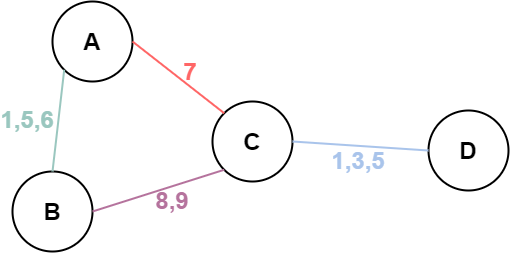
\includegraphics[scale=0.6]{images/temporal_graph_a.png}
    \caption{An static graph illustration of a temporal network.}
\end{figure}
\begin{figure}
    \centering
    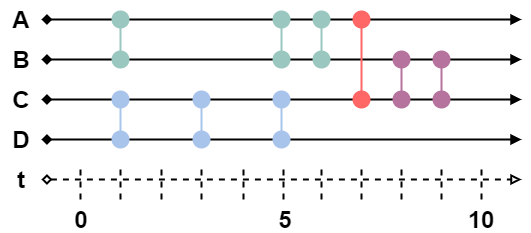
\includegraphics[scale=0.6]{images/temporal_graph_b.png}
    \caption{An timeline illustration of a temporal network.}
\end{figure}
The above figures illustrate a temporal network in two representations. The first figure is a static graph, with each edge labelled with the active/available times (time-edges/links). The second figure shows the timeline of the network, with the times-edges become available represented as connections between the node rows. The timeline representation better illustrates the temporal connectivity of the graph, while the static representation shows the structure of the network. Note that in the static graph, while node D is 'connected' to node A,B through C, it is in fact not possible to traverse from A/B to D, as the time-edges from C to D are, in a sense, too early. This indicates the lack of temporal information/intuition a static representation has, and further indicates that static and temporal networks are indeed fundamentally distinct.
Once a temporal graph is built, there are many measurements and algorithms that can be applied to the network in order to produce temporal metrics. Network latency, reachability and centrality are all distinctive properties of temporal networks, and can have a large impact on the performance of the network being modelled.\\
The research and interest in the domain of temporal networks is increasing as technology advances, and there is growing evidence \cite{social_metrics} that the modelling and analysis of such networks can produce useful results and information. Therefore, a convenient and purposeful library to enable this effort would be advantageous.
\end{introduction}
\vspace{1cm}
\clearpage

%--- Project Aim/Goal ---%
\begin{specification}
\section{Specification \& Aim}
The overall aim of the project is to build an open-source library that enables temporal network modelling and analysis in an intuitive, user-friendly and powerful manner. The library will also allow for multiple contributors to develop the project further, in an open-source environment. The specification of the library can be split into some key areas; core functionality, extendable functionality, selected language/platform and open-source setup.

\subsection{Core Functionality}
The core functionality of the library is divided into several items.
\begin{itemize}
    \item Input handling:\\
    Raw temporal data can be acquired and stored in a multitude of manners and formats. This is unsurprising considering the wide scope of temporal networks. It is therefore important that the library has the ability to handle multiple types of input while also allowing for new input handling methods to be added easily. There is also the possibility of having input data with no clear set of nodes or edges specified, that needs a conversion process to first decide the nodes \& edges, along with the time labels and other information. An example of this could be messaging logs from a social network, or a transport network timetable.
    \begin{table}[h!]
    \centering
        \begin{tabular}{ |c c c| }
        \hline
        CSV & GraphML & GEXF \\
        GDF & GML & XML \\
        \hline
        \end{tabular}
        \caption{Possible input formats \cite{graph_formats}.}
    \end{table}
    \item Graph creation/generation:\\
    The graph can be created in two ways; either from the post-processed input data, or a generated graph from a model. A generated graph could simply be a randomly generated set of time-edges labelled from within some probability distribution, or from a set of linear functions (s7,s8 \cite{intro_temporal}).
    \item Graph functions:\\
    There are multiple functions that can be developed once the graph has been created. These can range from selecting a node or edge, retrieving information from the graph/nodes/edges, adding/removing edges/nodes and so on. The graphs should also be save-able into a format which can be used to later recreate the graph. 
    \item Graph visualization:\\
    The created graph should be discernible in a intuitive and clear manner.
    \item Graph analysis:\\
    The user should be able to collect measurements on the graph, such as centrality, reachability and latency. The user should also be able to run and test algorithms on the graph, such as computing foremost time \cite{efficient_algorithms}.
    \item Output handling:\\
    Any metrics generated from the graph should be presentable in a report or file (.csv, for example).
\end{itemize}

\subsection{Extendable Functionality}
While the library will offer a lot of functionality, as described in the previous section, it is important for the design architecture to allow for easy extension from the core functionality. This is especially true in the case of an open-source project, where there is the possibility of contribution from the community. For example, if an individual wanted to add a new algorithm to calculate the shortest path, then this should be easily integrated in the current core library.

\subsection{Language \& Platform}
The selected language for this library is Python. Python is one of the most popular languages amongst developers and has many useful libraries on offer, such as numpy, matplotlib, scikit, pandas, tensorflow and more. All the source code and documentation will be hosted on GitHub, including this document, user-guides and readmes.\\
An important note is that this library is not aiming to be extremely efficient in order to handle large temporal graphs or data. A more appropriate choice of language for this would be C++. This library is essentially trying to emulate what NetworkX \cite{NetworkX} has achieved for static graphs, in terms of convenience, functionality and open-source, communal deployment.

\subsection{Open-source}
The idea of making a project open-source is powerful since it allows people to freely contribute to the project without the usual barriers to collaboration. If there is enough interest and motivation in the project domain, the library can develop rapidly. It also allows the users to freely modify and customize the library to suit their own needs and the needs of others. Any customization that could benefit the user base can be requested to be added as a permanent feature in the next release, improving the overall quality of the library. There are a number of important steps involved in launching a project as open-source \cite{open_source}.
\end{specification}
\vspace{1cm}
\clearpage

%--- Design ---%
\begin{design}
\section{Design Overview}
Based on the project specification, there are a number of important functions the library needs to provide. These functions can be summarized in a flowchart (figure 3). The following subsections will move down the flowchart, discussing the planned design and architecture of each component.
\begin{figure}[h]
    \centering
    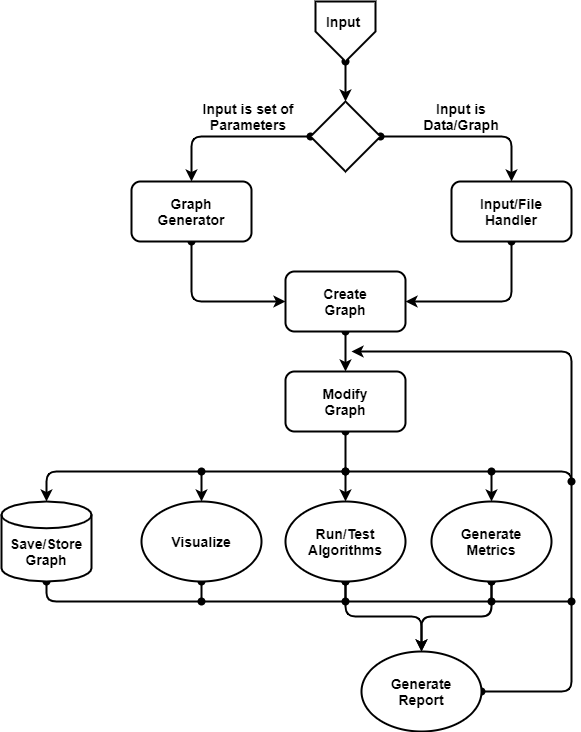
\includegraphics[scale=0.58]{images/flowchart.png}
    \caption{Functionality flowchart.}
\end{figure}
\subsection{Input}
The flowchart input can be of multiple types; raw temporal data that has been collected from a system, a previously created graph that was stored in a file, or a set of parameters for a graph generator. Given that there are expected to be many types of input formats, a modular approach to input handling is required. Each type of input should handled with a new subclass and produce the same set of outputs for graph creation. The parent input class should hold any properties and methods that are common across all inputs.
\subsection{File Handler}
Each file format will be handled by creating an input handler subclass from the input class. For example, if the input is a .csv file with a list of time-edges (figure 5), then this should be handled using the CSVInput class (figure 4).
\begin{figure}[h]
  \centering
  \begin{minipage}[b]{0.4\textwidth}
    \centering
    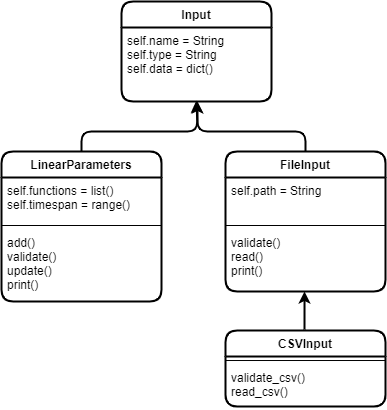
\includegraphics[scale=0.6]{images/UML_input.png}
    \caption{Example input handlers.}
  \end{minipage}
  \hfill
  \begin{minipage}[b]{0.4\textwidth}
    \centering
    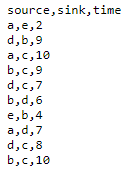
\includegraphics[scale=0.8]{images/csv.PNG}
    \caption{Sample csv file; list of time-edges.}
  \end{minipage}
\end{figure}
A common output format across the input handler classes would be very useful. This would allow for the construction of the graph to remain the same for an ambiguous set of inputs, as each input is handled within its own class. Any input validation unique to the input should also be added to this class, prior to passing the output to the graph constructor.
\subsection{Generators}
As mentioned in the specification, there are multiple methodologies available for generating temporal networks. Two examples are random generation of time-edges, and the generation of time-edges from a set of linear functions. Each generator would be defined as a class and produce the same output format  in order to remain compatible with the graph constructor. This allows an ambiguous set of generators to be created/defined without having to redesign the graph constructor for each.
\subsection{Graph Construction}
The construction of a temporal graph can be achieved in multiple ways. One idea is to simply store all the time-edges in a data structure, such as a dictionary, as a property of a temporal graph object. Another is to create a static graph for every instance of (discrete) time, or over a set of time intervals. These static snapshots could be represented in a class, and added into a data structure which would be stored as a property of the temporal graph object.\\
The chosen architecture looks at the temporal graph at a more granular level; modelling the components of the graph. Static graphs are built from nodes and edges, while temporal graphs are built from nodes and time-edges/links. The idea is that one could create a base class definition for nodes and edges, and then extend that definition to the temporal domain. Further extensions could also be realized for other graph constructions, custom specifications and use-cases.\\
This modular building block approach offers a flexible and powerful way of expressing a graph.
\begin{figure}[t]
    \centering
    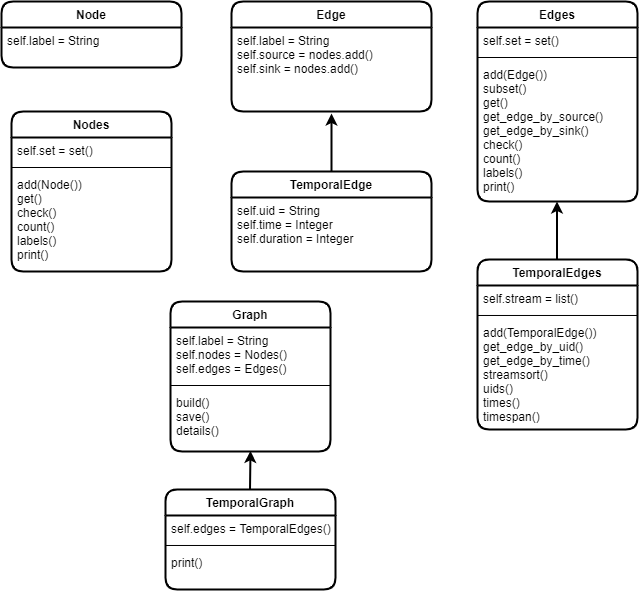
\includegraphics[scale=0.7]{images/UML_graph_components.png}
    \caption{Graph components and graph UML diagram.}
\end{figure}
Figure 6 shows some basic class definitions for the components of the Graph and TemporalGraph classes (digraph and discrete digraph respectively). A Graph has the properties nodes and edges, which are classes that define collections of the Node and Edge components, respectively. Nodes describes a set of Node objects, each of which has a label property. Similarly, the Edges describes a list of Edge objects, each of which has a label, source and sink property (here we are dealing with directed edges). The source and sink of an Edge object are Node objects themselves, stored in a Nodes collection. The idea here is that, when adding an Edge to a graph, the graph's Nodes collection is passed as a parameter, in order to maintain and update the graph's nodes. This process occurs in the constructor method of the Edge class.\\
For the TemporalGraph definition, the edges property is simply replaced with the TemporalEdges class, which is a subclass of the Edges class. TemporalEdges is a stream (list, ordered by time) of TemporalEdge objects. TemporalEdge is a subclass of Edge, with some new properties, such as uid (label name + time), time (discrete) and duration (discrete). By construction, the TemporalGraph class is already fundamentally different than that of the Graph class, which is expected and was mentioned in the introduction. When building the graph, the nodes and edges are connected through the node properties source and sink, while adding the edges themselves. Any unconnected nodes can then be added afterwards by directly calling the Nodes add() method. All the information required to build the graph will be passed from the input handler object data property (figure 4).
\subsection{Graph Functions}
The created graph can have a number of functions associated with the overall graph, and the components themselves. Typical graph functions include printing the graph details, and generating a visualization. The edges can be retrieved through methods like graph.edges.get\_edge\_by\_source('b'), graph.edges.get\_edge\_by\_sink('a'), graph.edges.get\_edge\_by\_time(3). Nodes can be retrieved through graph.nodes.get('x'). Each of these methods returns a new Edges/Nodes collection, which is a subset of the graph itself. All of the methods are callable on the subset. Figure 7 demonstrates this functionality.
\begin{figure}[h]
    \centering
    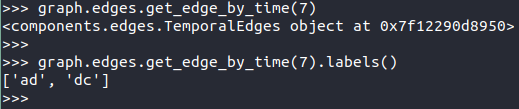
\includegraphics[scale=0.7]{images/graph_get_edge_labels.PNG}
    \caption{Graph functions example.}
\end{figure}

\subsection{Graph Modification}
New nodes and edges can be added to the graph through the respective add() functions of the collection classes. Similarly, nodes and edges should be removable from the graph, taking care to handle any unconnected edges. Furthermore, the properties of edges and nodes should be editable, provided the edit is valid and does not violate graph integrity or any added constraints. 
\subsection{Saving a Graph}
The Graph class includes a save() method, which will run through the graph components and save all structural information (basic save) into a file, including any new metrics generated during the session (full save). The file can also include a complete summary of the graph. By saving into a specified format, the graph should be reproducible from the file.
\subsection{Visualization}
It is important for the user to be able to visualize the graph, or subsections of the graph. Visualization can provide a means of quick verification by the user to see if the graph has been created or modified correctly. It can also aid in the verification of any results produced in testing. A simple command line means of visualization is shown in figure 8. Ultimately, the library would allow for circle \cite{circle_plot} and slice plots (figure 2) of the graph, by using the matplotlib package. The circle plots could be generated for each time step and then the images combined into a .gif format or played in sequence, to produce a dynamic plot of the network. Effective visualization may be challenging as larger networks become increasingly more complex. Some examples of circle and slice plots can be found at the teneto github \cite{teneto}, using a combination of circles and Bézier curves.
\clearpage
\begin{figure}[t]
    \centering
    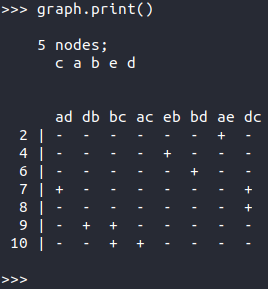
\includegraphics[scale=0.7]{images/graph_print.PNG}
    \caption{Text-based link activity matrix for a discrete temporal network.}
\end{figure}
\subsection{Algorithms \& Metrics}
The algorithm below calculates the foremost time and shortest path from the specified source node to all other nodes in the graph, between a specified time interval. As the algorithm moves through the time-ordered stream of the edges within the graph, the edge's foremost time is compared with the current stored time for the sink node (initialized at $\infty$), assuming that the edge start time and duration is within the specified interval. If the edge's foremost time is lower that the current stored one, the foremost time and the source node are updated in the foremost dictionary under the sink node's entry. This process continues until either the edge times are greater than the upper bound of the interval, or until all the edges have been processed.\\
\vspace{0.1cm}
\begin{algorithm}[H]
\SetAlgoLined
\caption{Foremost time/shortest path algorithm (s4.2 \cite{efficient_algorithms}, modified).}
\KwIn{An edge-stream representation of the graph, a time interval $(t_\alpha, t_\omega)$, a source node x.}
\KwOut{A dictionary of foremost times and previous nodes from the source node to the rest of the graph.}
 initialize $foremost[v][time]=\infty$ for all $v\ \epsilon\ V$, \\
 \hspace{1.5cm}$foremost[x][time]=t_\alpha$, and $foremost[x][source]=x$\;
 \ForEach{edge $e=(u, v, t, \lambda)$ in the edge stream}{
  \uIf{$t+\lambda \leq t_\omega$ and $t \geq t[u]$}{
    \uIf{$t+\lambda < t[v]$}{
        $t[v] \longleftarrow t+\lambda$\;
    }
  }
  \uElseIf{$t \geq t_\omega$}{
    break\;
  }
 }
 \Return{foremost[v][time], foremost[v][source] for each $v\ \epsilon\ V$}\;
\end{algorithm}
\vspace{0.1cm}
This example represents a typical case of the algorithms that will be added to the library for graph analysis, and was implemented in order to better understand what classes, properties and methods were required in the core library's architecture. Figure 9 shows the initial implementation, and figure 10 shows the resulting output. The inputs to the algorithm were the graph from figure 8, the source node 'a' and the total time span of the graph. The resulting dictionary provides a table of the foremost times from node 'a' to every other node in the graph (note: the duration of each edge is 1). For example, the earliest you can be at node 'c' from node 'a' is at time 8. This is achieved by moving along the path $(a \to e \to b \to d \to c )$. It can be noted by looking at the graph that there is another path from $(a \to d \to c)$, but this journey only arrives at node 'c' by time 9 and is therefore not the foremost path.
\clearpage
\begin{figure}[t]
  \centering
  \begin{minipage}[b]{0.4\textwidth}
    \centering
    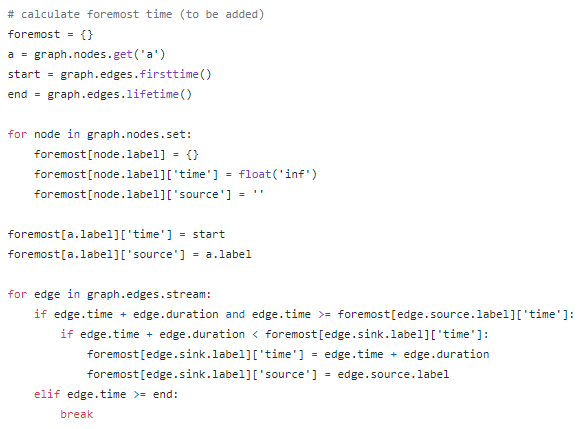
\includegraphics[scale=0.8]{images/foremost_code.PNG}
    \caption{Initial foremost time/shortest path implementation.}
  \end{minipage}
  \hfill
  \begin{minipage}[b]{0.4\textwidth}
    \centering
    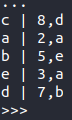
\includegraphics[scale=0.7]{images/foremost_result.PNG}
    \caption{Resulting dictionary.}
  \end{minipage}
\end{figure}
The finalized implementation would be wrapped in an algorithm subclass. The data structure for the result would be in the form of a temporal tree. Other algorithms for calculating network centrality, latency, connectivity and reachability could also be created as algorithm subclasses. Each of these subclasses would produce its respective metrics in a standardized format.
\subsection{Reports}
The results of any measurements and algorithms run/tested on the graph should be printable in an intuitive and clear format. This can be handled through a report class definition.
\subsection{Design Evaluation}
Verification of the code can be achieved by testing all the methods individually and by writing unit tests \cite{unittest}. Any algorithms implemented can be tested on a suitable test case temporal network and verified visually and through careful inspection. The test case network should be small enough to allow for easy verification, but complex enough to allow for good test coverage. An idea for a test case would be a transport network timetable.
\clearpage
\subsection{Open-source checklist}
\begin{itemize}
  \item Code:\\
  The code will be written in a consistent convention, such as the PEP8 style guide \cite{pep8}. The code should also be well commented, with a clear naming convention.
  \item Documentation:\\
  The library will be well-documented and include a readme, contributing, and code of conduct.
  \item License:\\
  The library will include a license file with a suitable open-source license.
  \item Library name:\\
  The name of the library will be easy to remember, relevant to the library domain and will not conflict with other libraries or trademarks.
  \item Further information about the guide being followed can be found at 'opensource.guide' \cite{open_source}.
\end{itemize}
\subsection{Notes}
\begin{itemize}
  \item Initial library:\\
  The initial library will be created for discrete time, directed temporal networks.
  \item Continuous time:\\
  The library can be expanded to deal with continuous time networks, time-permitting.
  \item Undirected/directed graphs:\\
  The above examples deal with directed graphs. Undirected graphs can be added to the library.
  \item Modular design:\\
  Overall, it is important to ensure the library is designed in a modular fashion, as there is the potential for multiple contributors to be working on it in the future. This also makes the library easier to maintain.
  \item Efficiency:\\
  Any methods implemented that perform some function on the network will be developed with efficiency in mind. The modelling and analysis of larger networks should not be grossly hindered by the library's performance.
\end{itemize}
\end{design}
\clearpage

%--- Project Plan ---%
\begin{plan}
\section{Project Plan}
\subsection{Planned deliverables}
The expected deliverables of the final project is as follows:
\begin{itemize}
  \item A functional library for the modelling and analysis of discrete time temporal networks, including:
  \begin{itemize}
      \item Multiple input handlers.
      \item Graph generation.
      \item Graph creation, modification and storage.
      \item Network analysis (core algorithms, metrics).
      \item Basic network visualization.
  \end{itemize}
  \item Showcase of one or more suitable test case temporal networks.
  \item Successful launch of the library as an open-source project on GitHub.
  \item A clear plan for the future development of the library.
\end{itemize}
\subsection{Timeline}
The project timeline is summarized in a Gantt chart\cite{gantt}.
The chart outlines the work completed and the next steps (week five is the current week of the project).
\begin{figure}[h]
    \centering
    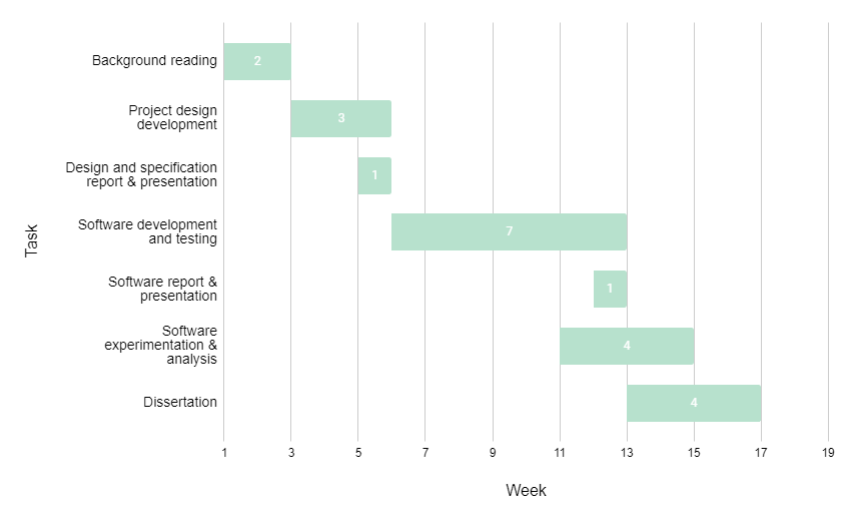
\includegraphics[scale=0.7]{images/timeline.PNG}
    \caption{Project timeline.}
\end{figure}
\clearpage
Figure 12 breaks down 'software development and testing', which is the next major phase of the project for the coming 7 weeks, before the next report is created.
\begin{figure}[h]
    \centering
    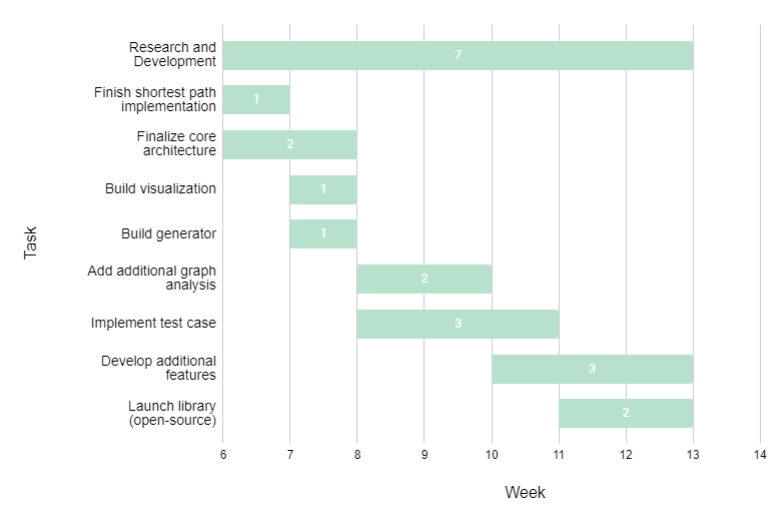
\includegraphics[scale=0.7]{images/dev_timeline.PNG}
    \caption{Software development and testing timeline (weeks 6-12).}
\end{figure}
\end{plan}
\vspace{1cm}
\clearpage

%--- Skills Acquired ---%
\begin{requirements}
\section{Requirements \& Skills}
\subsection{Software}
The library will be based on Python 3.7 and will require, at a minimum, the following packages:
\begin{itemize}
  \item NumPy - extended numerical computation capability \cite{numpy}.
  \item Matplotlib - visualization \cite{matplotlib}.
  \item Git - the project will be controlled and hosted through Git \cite{git} and GitHub \cite{github}, respectively.
\end{itemize}
\subsection{Data}
Temporal data will be required to fully test and showcase the libraries capabilities. An example of temporal data is the anonymous user messaging data-set from the Stanford University SNAP network analysis tool \cite{snap_data}. A transport network's timetable could also be used as a source of temporal data, for example a subsection of the London Tube service \cite{tube}.
Any data used in the project will be taken from the public domain. Sensitive data will be avoided as obtaining and verifying data compliance can be a time-consuming process and is not needed for the purposes of this project.
\subsection{Skills}
The skills required for successful completion of the project are as follows:
\begin{itemize}
  \item Strong programming skills for the development of object-oriented software.
  \item Experience in the Python programming language.
  \item Strong ability to effectively research a technical subject area.
  \item Strong mathematical and problem-solving ability.
  \item Experience of Git and GitHub.
  \item Strong time-management skills.
\end{itemize}
\subsection{Learning Outcomes}
The expected learning outcomes to be gained from the project are:
\begin{itemize}
    \item Effectively research, plan and execute a substantial project in the Computer Science domain.
    \item Further improve and develop programming, critical-thinking, problem-solving, mathematical and other technical skills.
    \item Build a high-quality software package through research, specification, design and planning.
    \item Launch an open-source project.
    \item Deliver technical, clear and concise documentation for both the MSc program and resulting library.
    \item Deliver high-quality formal presentations.
\end{itemize}
\end{requirements}
\vspace{1cm}
\clearpage

%--- Appendix ---%
%\begin{appendix}
\section*{Appendix}
\end{appendix}
\vspace{1cm}
\clearpage

%--- Bibliography ---%
\begin{thebibliography}{30}

\bibitem{graph_theory}
J. A. Bondy, Graph Theory With Applications. GBR: Elsevier Science Ltd., 1976.

\bibitem{stocks_example}
L. Zhao, G.-J. Wang, M. Wang, W. Bao, W. Li, and H. E. Stanley, ‘Stock market as temporal network’, Physica A: Statistical Mechanics and its Applications, vol. 506, pp. 1104–1112, Sep. 2018, doi: 10.1016/j.physa.2018.05.039.

\bibitem{wireless_example}
K. Römer, Temporal Message Ordering in Wireless Sensor Networks. 2002.

\bibitem{transport_example}
R. Gallotti and M. Barthelemy, ‘The multilayer temporal network of public transport in Great Britain’, Sci Data, vol. 2, no. 1, p. 140056, Dec. 2015, doi: 10.1038/sdata.2014.56.

\bibitem{social_example}
S. Lee, L. E. C. Rocha, F. Liljeros, and P. Holme, ‘Exploiting Temporal Network Structures of Human Interaction to Effectively Immunize Populations’, PLoS ONE, vol. 7, no. 5, p. e36439, May 2012, doi: 10.1371/journal.pone.0036439.

\bibitem{intro_temporal}
O. Michail, ‘An Introduction to Temporal Graphs: An Algorithmic Perspective’, arXiv:1503.00278 [cs], Mar. 2015, Accessed: Jun. 29, 2020. [Online]. Available: http://arxiv.org/abs/1503.00278.

\bibitem{graph_formats}
‘Supported Graph Formats’. https://gephi.org/users/supported-graph-formats/ (accessed Jun. 30, 2020).

\bibitem{efficient_algorithms}
H. Wu, J. Cheng, Y. Ke, S. Huang, Y. Huang, and H. Wu, ‘Efficient Algorithms for Temporal Path Computation’, IEEE Transactions on Knowledge and Data Engineering, vol. 28, no. 11, pp. 2927–2942, Nov. 2016, doi: 10.1109/TKDE.2016.2594065.

\bibitem{NetworkX}
‘NetworkX — NetworkX documentation’. https://networkx.github.io/ (accessed Jun. 30, 2020).

\bibitem{open_source}
‘Starting an Open Source Project’, Open Source Guides. https://opensource.guide/starting-a-project/ (accessed Jun. 30, 2020).

\bibitem{temporal_theory}
P. Holme and J. Saramäki, Eds., Temporal Network Theory. Springer International Publishing, 2019.

\bibitem{social_metrics}
J. Tang, M. Musolesi, C. Mascolo, and V. Latora, ‘Temporal distance metrics for social network analysis’, in Proceedings of the 2nd ACM workshop on Online social networks, Barcelona, Spain, Aug. 2009, pp. 31–36, doi: 10.1145/1592665.1592674.

\bibitem{unittest}
‘unittest — Unit testing framework — Python 3.8.4rc1 documentation’. https://docs.python.org/3/library/unittest.html (accessed Jul. 02, 2020).

\bibitem{gantt}
B. Gavin, ‘How to Create a Gantt Chart in Google Sheets’, How-To Geek. https://www.howtogeek.com/447783/how-to-create-a-gantt-chart-in-google-sheets/ (accessed Jul. 02, 2020).

\bibitem{circle_plot}
‘circularGraph’. https://www.mathworks.com/matlabcentral/fileexchange/48576-circulargraph (accessed Jul. 02, 2020).

\bibitem{numpy}
‘NumPy’. https://numpy.org/ (accessed Jul. 02, 2020).

\bibitem{matplotlib}
‘Matplotlib: Python plotting — Matplotlib 3.2.2 documentation’. https://matplotlib.org/index.html (accessed Jul. 02, 2020).

\bibitem{snap_data}
‘SNAP: Network datasets: CollegeMsg temporal network’. https://snap.stanford.edu/data/CollegeMsg.html (accessed Jul. 02, 2020).

\bibitem{tube}
T. for L. | E. J. Matters, ‘Timetables’, Transport for London. https://www.tfl.gov.uk/travel-information/timetables/ (accessed Jul. 02, 2020).

\bibitem{git}
‘Git’. https://git-scm.com/ (accessed Jul. 02, 2020).

\bibitem{github}
‘Build software better, together’, GitHub. https://github.com (accessed Jul. 02, 2020).

\bibitem{pep8}
‘PEP 8 -- Style Guide for Python Code’, Python.org. https://www.python.org/dev/peps/pep-0008/ (accessed Jul. 02, 2020).

\end{thebibliography}
\vspace{1cm}

\end{document}